\documentclass[10pt]{report}
\usepackage{epsf}
\usepackage{amsmath}
\usepackage{amssymb}
\usepackage{float}
\usepackage{palatino}
\usepackage[pdftex]{graphics}
\usepackage{fancyhdr}
\usepackage[pdftex]{graphicx}
\usepackage{hyperref}
\parindent 0in
\parskip 1ex
\oddsidemargin  0in
\evensidemargin 0in
\textheight 8.5in
\textwidth 6.5in
\topmargin -0.25in

\pagestyle{fancy}
\fancyhf{}
\fancyhead[L]{\bf BME354L - Palmeri - Spring 2013}
\fancyhead[R]{{\bf Arduino Project}}
%\fancyfoot[L]{LICENSE: CC BC-NC-SA 3.0 ({\tt http://creativecommons.org/licenses/by-nc-sa/3.0/})}
\fancyfoot[C]{\thepage}

\title{Tips for Using Thermocouples}
\author{Will Scheideler}
\begin{document}

\section*{Tips for Using Thermocouples}

\subsection*{Introduction}
A thermocouple is a transducer used to convert a temperature to a voltage. Thermocouples are manufactured in a number of varieties (Type J, K, T, etc), with specific applications for each. The voltage produced by the thermocouple is a function of the material properties (the work functions of each metal in the bimetallic junction) of the sensing element, as well as the temperature. Each thermocouple variety has an optimal operating range of temperatures. For monitoring the temperature range of the reflow oven, we have chosen a type K thermocouple (chromel-alumel), which can effectively sense the range of temperatures for this application (50C – 250 C).

\par
	The output voltage of a thermocouple is proportional to temperature. However, reading the output of the thermocouple requires some careful signal conditioning. The sensitivity of a Type K thermocouple is approximately 41 $\mu$V/°C. This means that significant amplification is required to achieve measurable differences in the output voltage over the relevant temperature range. This amplification could be easily accomplished with an instrumentation amplifier (excellent CMRR, easily tunable gain, etc). However, there is an additional requirement of the signal conditioning circuit. The thermocouple is not linear over a wide range of temperatures. This means that the transfer function relating Output voltage to Temperature is non-linear (Guess what this shape would be from your knowledge of thermistors). 

\subsection*{AD8495}
	There are a variety of commercially available integrated circuits that are useful for simultaneously amplifying and linearizing the thermocouple output voltage signal. For our application, we have chosen the AD8495, which is optimized for use with a Type K thermocouple. This chip provides a cold junction reference internally, which can allow for absolute temperature measurements(This reference voltage would otherwise be provided by an ice-temperature reference). 
\par
	The pin diagram and assignments are detailed below. You can see that this chip resembles the packaging of the AD620 and INA126 instrumentation amplifiers which you have used in lab. There are two pins (IN-  /  IN+) for the differential inputs to this chip, which are intended to be connected to the two ports of the Type-K thermocouple. The AD8495 is effectively an instrumentation amplifier that has been optimized for this particular application with lazer resistor trimming to precisely set the gain. This gain has been tuned to provide an output that is precisely $5 mV/°C$. (Can you guess why this particular value is chosen? Think about the Vlsb of the 10 bit ADC on the Arduino Board.)

\begin{figure}[H]
\centering
   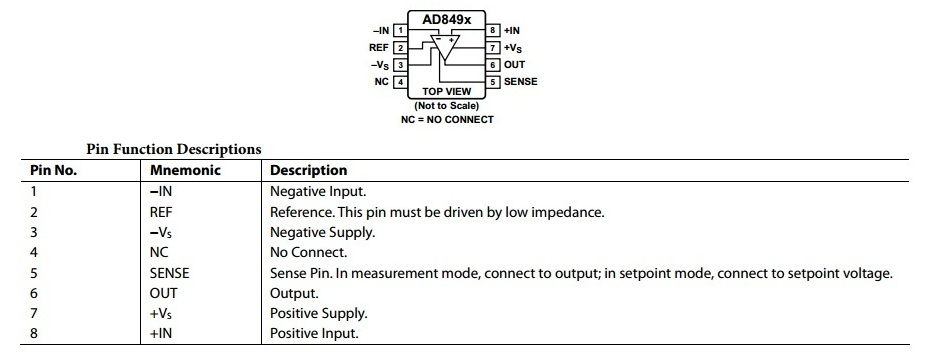
\includegraphics[width=0.7\textwidth]{AD8495_Pins.jpg}
    \caption{AD8495 Pin Diagram}
\end{figure}

\subsection*{Thermocouple Circuit}
	The circuit shown below shows an implementation of the AD8495 as a signal conditioning circuit for the Type-K thermocouple. Notice a few important features of this implementation. The AD8495 has a reference voltage that is used to compute its differential output voltage (labeled as AREF below). This value can be used to set the output voltage range of this chip (Consider how you could improve the sensitivity of your analog to digital conversion by using this reference?). We have made this reference voltage tunable with a potentiometer. The AD8495 is powered in a single-supply configuration (Vdd = 5V, Vss = GND) so that it may be powered directly from the Arduino. See Single Supply OpAmps for a detailed description of single supply applications.
 \par
	The other feature in the circuit shown below is the OMRON G3NE solid-state relay. The OMRON relay, shown below as Relay1, is used to switch power to the reflow oven ON and OFF. The relay is activated by applying a HIGH voltage to the control pins (P/S). When the relay is activated, it can conduct up to 20A of AC current (between pins 1 and 2) to supply the oven. When the relay is in the OFF state, no power flows to the reflow oven heating elements. The Arduino is used to supply the control signal for the relay (If the input impedance of the relay control is 300Ω, how much current will the output pin of the Arduino need to provide?). The other important behavior of the solid-state relay is that it will not be able to switch off while carrying a high AC current (an intrinsic property of the silicon controlled rectifiers used to construct the relay). This is useful for our purposes since it precludes the large current / voltage spikes that can occur when switching a mechanical relay during the middle of an AC cycle.
\par
	There are a few other common features in this circuit that you should note. Notice the 10 uF and the .1 uF capacitors that are attached to the Vdd supply to the AD8495. These are known as ‘decoupling capacitors.’ Decoupling capacitors are used to eliminate high frequency noise present on the voltage supplies to the AD8495. They are an essential feature in many circuits used to condition low level signals ($\mu V$ to $mV$ range).


\begin{figure}[H]
\centering
   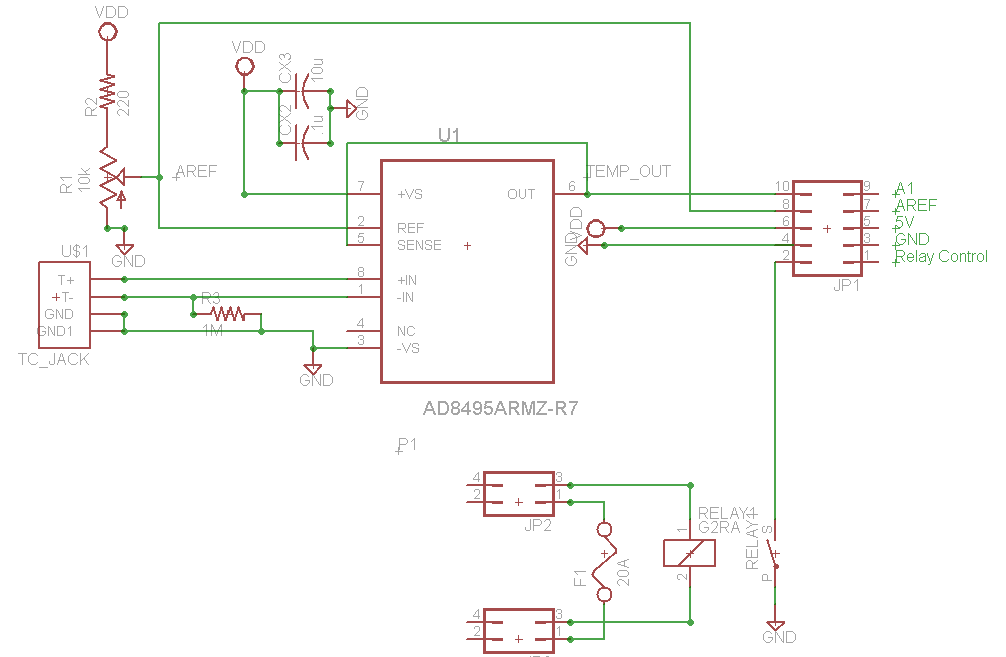
\includegraphics[width=0.8\textwidth]{Thermocouple_Circuit.png}
    \caption{Schematic of thermocouple circuit with built-in cold-junction refrence.}
\end{figure}


\end{document}